\section{Đề ôn thi giữa kỳ 2 toán 10}
\subsection{Phần trắc nghiệm}
Câu trắc nghiệm nhiều phương án lựa chọn. Học sinh trả lời từ
câu 1 đến câu 12. Mỗi câu hỏi học sinh \textit{chỉ chọn một} phương án.

\Opensolutionfile{ans}[Ans/Dapan]
\hienthiloigiaiex
\begin{ex}%[0D8V1-1]
	Một lớp có $23$ học sinh nữ và $17$ học sinh nam. Hỏi có bao nhiêu cách chọn một học sinh tham gia cuộc thi tìm hiểu môi trường?
	\choice
	{$23$}
	{$17$}
	{\True$40$}
	{$391$}
	\loigiai{
		Việc chọn một học sinh có hai trường hợp sau:
		\begin{enumerate}[TH1.]
			\item Người được chọn là nam: có $17$ cách.
			\item Người được chọn là nữ: có $23$ cách.
		\end{enumerate}
		Vậy theo quy tắc cộng, có $17+23=40$ cách chọn.
	}
\end{ex}
\begin{ex}%[0D8V1-2]
	Một lớp có $23$ học sinh nữ và $17$ học sinh nam. Hỏi có bao nhiêu cách chọn hai học sinh tham gia hội trại với điều kiện có cả nam và nữ?
	\choice
	{$40$}
	{\True$391$}
	{$780$}
	{$1560$}
	\loigiai{
		Việc chọn ra hai bạn có cả nam và nữ được thực hiện qua hai bước sau:\begin{enumerate}[Bước 1.]
			\item Chọn $1$ bạn nam: có $17$ cách.
			\item Chọn $1$ bạn nữ: có $23$ cách.
		\end{enumerate}
		Vậy theo quy tắc nhân, có tất cả $17\cdot23=391$ cách chọn.
	}
\end{ex}  
\begin{ex}%[0D8V1-4]
	Từ các chữ số $0$, $1$, $2$, $3$, $4$, $5$ có thể lập được bao nhiêu số có ba chữ số khác nhau và chia hết cho $3$?
	\choice
	{$36$}
	{$42$}
	{\True$40$}
	{$72$}
	\loigiai{
		Gọi số được lập đó là $\overline{abc}$ với $a,b,c\in\{0;1;2;3;4;5\}$ và $a\ne0$. Vì $\overline{abc}\,\vdots\,3$ nên $(a+b+c)\,\vdots\,3$, suy ra trong ba số $a$, $b$, $c$, có một số chia hết cho $3$, có một số chia $3$ dư $1$, và có một số chia $3$ dư $2$. Việc chọn ra số $\overline{abc}$ được thực hiện qua các trường hợp sau:\begin{enumerate}[TH1.]
			\item Tính cả trường hợp $a=0$ và $a\ne0$.\begin{enumerate}[Bước 1.]
				\item Chọn một số chia hết cho $3$: có $2$ cách.
				\item Chọn một số chia $3$ dư $1$: có $2$ cách.
				\item Chọn một số chia $3$ dư $2$: có $2$ cách.
				\item Sắp xếp $3$ chữ số vừa tìm theo thứ tự: có $3!$ cách.
			\end{enumerate}
			Vậy theo quy tắc nhân, TH1 có $2^3\cdot3!=48$ cách chọn.
			\item Xét trường hợp $a=0$.\begin{enumerate}[Bước 1.]
				\item Chọn một số chia $3$ dư $1$: có $2$ cách.
				\item Chọn một số chia $3$ dư $2$: có $2$ cách.
				\item Sắp xếp $2$ số vừa tìm được theo thứ tự: có $2!$ cách.
			\end{enumerate}
			Vậy theo quy tắc nhân, TH2 có $2^2\cdot2!=8$ cách chọn.
		\end{enumerate}
		Từ đó suy ra, có $48-8=40$ số thoả mãn.
	}
\end{ex}
\begin{ex}%[0D8V2-3]
	Từ các số thuộc tập $A=\{1;2;3;4;5;6;7\}$ có thể lập được bao nhiêu số tự nhiên có bốn chữ số khác nhau và chia hết cho $5$?
	\choice
	{$360$}
	{\True$120$}
	{$480$}
	{$347$}
	\loigiai{
		Gọi số cần lập là $\overline{abcd}$ với $a,b,c,d\in A$. Vì $\overline{abcd}\,\vdots\,5$ nên $d=5$. Ta chỉ cần chọn $3$ số trong $6$ số $1$, $2$, $3$, $4$, $6$, $7$ để xếp vào $3$ vị trí $a$, $b$, $c$. Do đó ta có tất cả $\mathrm{A}^3_6=120$ số thoả mãn.
	}
\end{ex}
\begin{ex}%[0D8V2-4]
	Có bao nhiêu cách chọn và sắp xếp thứ tự $5$ cầu thủ để đá luân lưu $11$ mét? (Biết rằng $11$ cầu thủ có khả năng được đá luân lưu như nhau).
	\choice
	{\True$55440$}
	{$20680$}
	{$32456$}
	{$41380$}
	\loigiai{
		Chọn ra $5$ cầu thủ trong $11$ cầu thủ và sắp xếp theo thứ tự có $\mathrm{A}^5_{11}=55440$ cách chọn.
	}
\end{ex}
\begin{ex}%[0D8V3-4]
	Số hạng không chứa $x$ trong khai triển nhị thức Newton của $\left(\sqrt{x}+\dfrac{3}{x}\right)^3$ là
	\choice 
	{$4$}
	{\True$9$}
	{$6$}
	{$-4$}
	\loigiai{
		Số hạng tổng quát của khai triển có dạng $\mathrm{C}^k_n\left(\sqrt{x}\right)^{3-k}\left(\dfrac{3}{x}\right)^k=\mathrm{C}^k_n3^kx^{-\frac{3}{2}k+\frac{3}{2}}$. Do số hạng không chứa $x$ nên ta suy ra $-\dfrac{3}{2}k+\dfrac{3}{2}=0$ hay $k=1$. Do đó số hạng cần tìm là $\mathrm{C}^1_33^1x^0=9$.
	}
\end{ex}
\begin{ex}%[0H9H1-3]
	Véc-tơ $\vec{a}=(-4;0)$ được phân tích theo hai véc-tơ đơn vị như thế nào?
	\choice 
	{$\vec{a}=-4\vec{i}+\vec{j}$}
	{$\vec{a}=-\vec{i}+4\vec{j}$}
	{$\vec{a}=-4\vec{j}$}
	{\True$\vec{a}=-4\vec{i}$}
	\loigiai{
		Ta có $\vec{a}=(-4;0)\Leftrightarrow\vec{a}=-4\vec{i}+0\vec{j}=-4\vec{i}$.
	}
\end{ex}
\begin{ex}%[0H9H1-4]
	Mệnh đề nào sau đây đúng?
	\choice 
	{Hai véc-tơ $\vec{u}=(2;-1)$ và $\vec{v}=(-1;2)$ đối nhau}
	{Hai véc-tơ $\vec{u}=(2;-1)$ và $\vec{v}=(-2;-1)$ đối nhau}
	{\True Hai véc-tơ $\vec{u}=(2;-1)$ và $\vec{v}=(-2;1)$ đối nhau}
	{Hai véc-tơ $\vec{u}=(2;-1)$ và $\vec{v}=(2;1)$ đối nhau}
	\loigiai{Ta có véc-tơ đối của véc-tơ $\vec{u}=(2;-1)$ là $\vec{v}=-\vec{u}=(-2;1)$.
	}
\end{ex}
\begin{ex}%[0H9H1-3]
	Cho tam giác $ABC$ có trọng tâm là gốc toạ độ $O$, hai đỉnh $A$ và $B$ có toạ độ là $A(-2;2)$ và $B(3;5)$. Toạ độ của đỉnh $C$ là
	\choice 
	{$(1;7)$}
	{\True$(-1;-7)$}
	{$(-3;-5)$}
	{$(2;-2)$}
	\loigiai{
		Do $O$ là trọng tâm của tam giác $ABC$ nên ta có $\heva{&0=\dfrac{x_A+x_B+x_C}{3}\\&0=\dfrac{y_A+y_B+y_C}{3}}$. Từ đó suy ra $\heva{&x_C=-x_A-x_B=2-3=-1\\&y_C=-y_A-y_B=-2-5=-7}$ hay $C=(-1;-7)$.
	}
\end{ex}
\begin{ex}%[0H9H1-4]
	Cho hai điểm $A(1;0)$ và $B(0;-2)$. Toạ độ điểm $D$ sao cho $\vec{AD}=-3\vec{AB}$ là
	\choice 
	{$(4;-6)$}
	{$(2;0)$}
	{$(0;4)$}
	{\True$(4;6)$}
	\loigiai{
		Giả sử $D(x_D;y_D)$, do $\vec{AD}=-3\vec{AB}$ nên ta có $\heva{&x_D-x_A=-3(x_B-x_A)\\&y_D-y_A=-3(y_B-y_A)}$. Từ đó suy ra $\heva{&x_D=-3(x_B-x_A)+x_A=-3(0-1)+1=4\\&y_D=-3(y_B-y_A)+y_A=-3(-2-0)+0=6}$ hay $D(4;6)$.
	}
\end{ex}
\begin{ex}%[0H9H3-2]
	Trong mặt phẳng toạ độ $Oxy$, cho đường thẳng $d:\heva{&x=-2t\\&y=4+t}$. Trong các véc-tơ sau, véc-tơ nào là véc-tơ pháp tuyến của $d$?
	\choice 
	{$\vec{u}=(-2;1)$}
	{$\vec{v}=(2;-1)$}
	{$\vec{m}=(1;-2)$}
	{\True$\vec{n}=(1;2)$}
	\loigiai{
		Đường thẳng $d$ nhận véc-tơ $\vec{u}=(-2;1)$ làm véc-tơ chỉ phương, nên ta loại trừ phương án A. Mặt khác, ta có $\vec{n}\cdot\vec{u}=1\cdot(-2)+2\cdot1=0$ nên $\vec{n}$ vuông góc với $\vec{u}$. Do đó $\vec{n}=(1;2)$ là véc-tơ pháp tuyến của đường thẳng $d$.
	}
\end{ex}
\begin{ex}%[0H9V3-5]
	\immini{Trong mặt phẳng toạ độ $Oxy$, cho điểm $M$ và đường thẳng $\Delta$ như hình bên. Gọi $H$ là hình chiếu của $M$ lên đường thẳng $\Delta$. Độ dài đoạn thẳng $MH$ là
		\choice 
		{\True$2$}
		{$4$}
		{$2\sqrt{5}$}
		{$10$}
	}{
		\begin{tikzpicture}[scale=1, font=\footnotesize, line join=round, line cap=round, >=stealth]
			\pgfmathsetmacro\a{(asin(0.6)}
			\pgfmathsetmacro\b{(.25}
			\draw[->](-1.5,0)--(5.5,0)node[above]{$x$};
			\draw[->](0,-1.5)--(0,5)node[left]{$y$};
			\clip (-1.5,-1.5)rectangle(5.5,5);
			\draw[smooth]plot[domain=-4:6](\x,{-0.75*\x+3});
			\path 
			(2,4)coordinate(M)
			(0.8,2.4)coordinate(H)
			(0,0)coordinate(O)
			;
			\draw[dashed]
			(M)--(H)
			(0,4)-|(2,0)
			(-1.3,3.7)node{$\Delta$}
			;
			\draw(H)++(-\a:\b)--++(-\a+90:\b)--++(-\a+180:\b);
			\foreach \p/\g in {M/45,H/-135,O/-45} \fill[black](\p)circle(1pt)node[shift={(\g:.3)}]{$\p$};
			\foreach \p in {-3,-2,-1,1,2,3,4,5} \draw($(\p,0)+(0,1.5pt)$)--++(0,-3pt)node[below]{$\p$};
			\foreach \p in {-1,1,2,3,4} \draw($(0,\p)+(1.5pt,0)$)--++(-3pt,0)node[left]{$\p$};
	\end{tikzpicture}}
	\loigiai{
		Phương trình đường thẳng $\Delta$ đi qua hai điểm $(4;0)$ và $(0;3)$ là $\dfrac{x}{4}+\dfrac{y}{3}=1$ hay $3x+4y-12=0$. Độ dài $MH$ chính là khoảng cách từ $M$ đến đường thẳng $\Delta$, do đó ta được $$MH=\mathrm{d}_{(M,\Delta)}=\dfrac{\left|3\cdot2+4\cdot4-12\right|}{\sqrt{3^2+4^2}}=2.$$
	}
\end{ex}
\Closesolutionfile{ans}
\bangdapan{Dapan}

\subsection{Câu trắc nghiệm đúng sai}
Học sinh trả lời từ câu 1 đến câu 4.
Trong mỗi ý \circlenum{A}, \circlenum{B}, \circlenum{C} và \circlenum{D} ở mỗi câu, học sinh chọn đúng hoặc sai.
\setcounter{ex}{0}
\LGexTF
\Opensolutionfile{ansbook}[ansbook/DapanDS]
\Opensolutionfile{ans}[Ans/DapanT]
\begin{ex}%[0D8H2-4]% Đỗ Chí Tâm,dự án tex hóa đề 10,11
	Từ một nhóm $30$ học sinh khối $12$ gồm $15$ học sinh khối A, $10$ học sinh khối B và $5$ học sinh khối C, cần chọn ra $15$ học sinh. Khi đó,
	\choiceTF
	{số cách chọn để số học sinh mỗi khối là bằng nhau là $252\,252$}
	{\True số cách chọn để có $2$ học sinh khối C và $13$ học sinh khối B hoặc khối $A$ là $\mathrm{C}_5^2 \mathrm{C}_{25}^{13}$}
	{\True số cách chọn để có $2$ học sinh khối C, $10$ học sinh khối B và $3$ học sinh khối A là $\mathrm{C}_5^2 \mathrm{C}_{10}^{10} \mathrm{C}_{15}^{3}$ }
	{số cách chọn để có ít nhất $5$ học sinh khối A và có đúng $2$ học sinh khối C là $51\,861\,950$} 
	\loigiai{
		\begin{itemize}
			\item Số cách chọn để số học sinh mỗi khối bằng nhau là $\mathrm{C}_{15}^5 \mathrm{C}_{10}^5 \mathrm{C}_5^5=756\,756.$
			\item Chọn $2$ học sinh khối C có $\mathrm{C}_{5}^2$ cách.\\
			Chọn $13$ học sinh khối $B$ hoặc khối A có $\mathrm{C}_{25}^{13}$ cách.\\
			Vậy có  $\mathrm{C}_5^2 \mathrm{C}_{25}^{13}$ cách chọn thỏa yêu cầu bài toán.
			\item Số cách chọn để có $2$ học sinh khối C, $10$ học sinh khối B và $3$ học sinh khối A là $\mathrm{C}_5^2 \mathrm{C}_{10}^{10} \mathrm{C}_{15}^{3}$ cách.
			\item Số cách chọn $15$ học sinh, trong đó có đúng $2$ học sinh khối C là $\mathrm{C}_{5}^2 \mathrm{C}_{25}^{13}$.\\
			Số cách chọn $15$ học sinh, trong đó có đúng $2$ học sinh khối C và có không quá $4$ học sinh khối A là $\mathrm{C}_{15}^3 \mathrm{C}_5^2 \mathrm{C}_{10}^{10}+\mathrm{C}_{15}^4 \mathrm{C}_5^2 \mathrm{C}_{10}^{9}$.\\
			Vậy có $\mathrm{C}_{5}^2 \mathrm{C}_{25}^{13}-\left(\mathrm{C}_{15}^3 \mathrm{C}_5^2 \mathrm{C}_{10}^{10}+\mathrm{C}_{15}^4 \mathrm{C}_5^2 \mathrm{C}_{10}^{9}\right)=51\,863\,640$ cách chọn thỏa yêu cầu bài toán.
		\end{itemize}
	}
\end{ex}

\begin{ex}%[0D8N3-3]% Đỗ Chí Tâm,dự án tex hóa đề 10,11
	Khai triển $(3x+1)^4$. Khi đó,
	\choiceTF
	{\True hệ số của $x^4$ trong khai triển là $81$}
	{hệ số của $x^3$ trong khai triển là $118$}
	{\True hệ số của $x^2$ trong khai triển là $54$}
	{hệ số của $x$ trong khai triển là $1$}
	\loigiai{
		Ta có $(3x+1)^4=\mathrm{C}_4^0(3x)^4.1^0+\mathrm{C}_4^1(3x)^3\cdot 1^1+\mathrm{C}_4^2(3x)^2\cdot 1^2+\mathrm{C}_4^3(3x)\cdot 1^3+\mathrm{C}_4^4(3x)^0\cdot 1^4$.\\
		Do đó $(3x+1)^4=81x^4+108x^3+54x^2+12x+1$. Vậy
		\begin{itemize}
			\item hệ số của $x^4$ trong khai triển là $81$.
			\item hệ số của $x^3$ trong khai triển là $108$.
			\item hệ số của $x^2$ trong khai triển là $54$.
			\item hệ số của $x$ trong khai triển là $12$.
		\end{itemize}
	}
\end{ex}

\begin{ex}%[0H9V1-4]% Đỗ Chí Tâm,dự án tex hóa đề 10,11
	Trong mặt phẳng tọa độ $(Oxy)$, cho $3$ điểm $A(-2;-1),B(1;3),C(2;-3)$. Khi đó, 
	\choiceTF
	{\True $A,B,C$ là ba đỉnh của một tam giác}
	{điểm $I(0;-2)$ là trung điểm của $AB$}
	{điểm $M$ thuộc $Ox$ sao cho $AM+BM$ bé nhất có hoành độ bằng $\dfrac{5}{4}$}
	{điểm $N$ thộc $Oy$ sao cho $BN+CN$ bé nhất có tung độ bằng $2$}
	\loigiai{
		\begin{itemize}
			\item Ta có $\vec{AB}=(3;4), \vec{AC}=(4;-2);$ vì $\dfrac{3}{3}\ne \dfrac{4}{-2}\Rightarrow \vec{AB}$ và $\vec{AC}$ không cùng phương.\\
			Vậy ba điểm $A,B,C$ không thẳng hàng hay $A,B,C$ là ba đỉnh của một tam giác.
			\item Trung điểm của $A,B$ là $I \left( \dfrac{-1}{2};1\right)$.
			\item Do $y_A\cdot y_B=(-1)\cdot 3<0$ nên hai điểm $A,B$ nằm khác phía so với $Ox$.\\
			$M\in Ox$ để $AM+BM$ nhỏ nhất $\Rightarrow A,B,M$ thẳng hàng $\Rightarrow \vec{AB}$ và $\vec{AM}$ cùng phương.\\
			Gọi $M(x;0)\in Ox\Rightarrow \vec{AM}=(x+2;1)$ và $\vec{AB}=(3;4)$.\\
			Ta có $\vec{AM},\vec{AB}$ cùng phương $\Rightarrow \dfrac{x+2}{3}=\dfrac{1}{4}\Rightarrow x=-\dfrac{5}{4}$.\\
			Vậy $M \left(-\dfrac{5}{4};0 \right)$.
			\item Do $x_B\cdot x_C>0$ nên hai điểm $B,C$ nằm cùng phía đối với trục $Oy$.\\
			Lấy $C'$ đối xứng với $C$ qua $Oy$ suy ra $C'(-2;-3)$ ($C'$ và $B$ khác phía so với $Oy$).\\
			Vì $N$ thuộc $Oy$ nên $CN=C'N$. Do đó $BN+CN=BN+C'N$; tổng này bé nhất khi và chỉ khi $B,N,C'$ thẳng hàng hay $\vec{BC'},\vec{BN}$ cùng phương.\\
			Gọi $N(0;y)\in Oy\Rightarrow \vec{BN}=(-1;y-3),\vec{BC'}=(-3;-6)$.\\
			Ta có $\vec{BC'},\vec{BN}$ cùng phương $\Rightarrow \dfrac{-1}{-3}=\dfrac{y-3}{-6}\Rightarrow y=1$.\\
			Vậy $N(0;1)$.  
		\end{itemize}
	}
\end{ex}

\begin{ex}%[0H9V3-2]% Đỗ Chí Tâm,dự án tex hóa đề 10,11
	Trong mặt phẳng tọa độ $(Oxy)$, cho hình chữ nhật $ABCD$ có tâm $I(6;2)$ và các điểm $M(1;5), N(3;4)$ lần lượt thuộc các đường thẳng $AB,BC$. Biết rằng trung điểm $E$ của cạnh $CD$ thuộc đường thẳng $\Delta\colon x+y-5=0$ và hoành độ điểm $E$ nhỏ hơn $7$. Khi đó,
	\choiceTF
	{\True phương trình $BC$ là $x-3=0$}
	{phương trình $AB$ là $x+y-6=0$}
	{\True tọa độ điểm $A(9;5)$}
	{tọa độ điểm $B(3;3)$}
	\loigiai{
		\begin{center}
			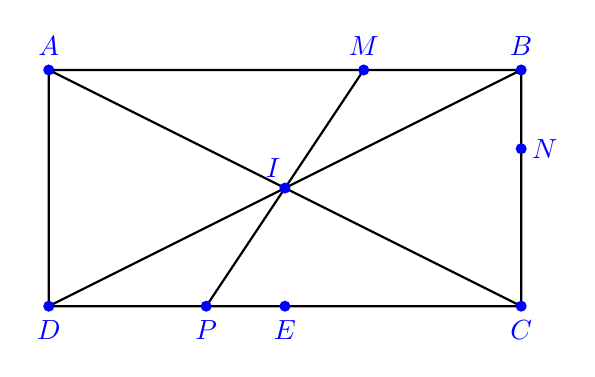
\begin{tikzpicture}[thick]
				%\draw[gray!20] (-3,-2) grid (6,5);
				\path (0,3) coordinate (A)  
				(6,3) coordinate (B)
				(0,0) coordinate (D)
				(6,0) coordinate (C)
				(3,0) coordinate (E)
				(4,3) coordinate (M)
				(6,2) coordinate (N)
				(3,1.5) coordinate (I)
				(2,0) coordinate (P);
				\draw (A)--(B)--(C)--(D)--(A) (M)--(P) (A)--(C) (B)--(D);
				\foreach \p/\q in {A/90, B/90, C/-90, D/-90, N/0,M/90,P/-90,E/-90,I/120}
				\fill[blue] (\p) circle(2pt) node[shift={(\q:3mm)}]{$\p$};
			\end{tikzpicture}
		\end{center}
		Gọi $P$ là điểm đối xứng với $M(1;5)$ qua $I(6;2)\Rightarrow P(11;-1)$ và $P$ thuộc đường thẳng $CD$.\\
		Ta có $E\in \Delta$ nên giả sử $E(t;5-t)$. Khi đó $\vec{IE}=(t-6;3-t), \vec{PE}=(t-11;6-t)$.\\
		Vì $E$ là trung điểm $CD$ nên $IE \bot PE$. Do đó, ta có\\
		\hspace*{1.5cm} $\vec{IE}\cdot \vec{PE}=0\Leftrightarrow (t-6)(t-11)+(3-t)(6-t)=0\Leftrightarrow t^2-13t+42=0$.\\
		Suy ra $t=6$ hoặc $t=7$.  Vì hoành độ của $E$ nhỏ hơn $7$ nên $E(6;-1)$.\\
		$BC$ đi qua $N(3;4)$ và vuông góc với $CD$ nên phương trình $BC$ là $x-3=0$.\\
		$AB$ đi qua $M(1;5)$ và song song với $CD$ nên phương trình $AB$ là $ y-5=0$.\\
		Từ phương trình các cạnh tìm được, ta có: $A(9;5), B(3;5),C(3;-1),D(9;-1)$.
	}
\end{ex}
\Closesolutionfile{ans}
\Closesolutionfile{ansbook}

\begin{center}
	\textbf{\textsf{BẢNG ĐÁP ÁN ĐÚNG SAI}}
\end{center}
\input{Ansbook/DapanDS}

\subsection{Phần tự luận}
\hienthiloigiaibt

%%%=============BT_1=============%%%
\begin{bt}%[0D8N2-3]%[Dự án đề kiểm tra Toán khối 10 GHKII NH23-24-Dot 2-Nguyễn Sĩ Đạt]%[Deso8-Sach CD]
	Có bao nhiêu số tự nhiên có năm chữ số, sao cho mỗi số đó, chữ số đứng sau lớn hơn chữ số chữ số đứng trước?
	\loigiai{
	Vì chữ số đầu tiên của số tự nhiên phải khác $0$, các chữ số đứng sau lớn hơn chữ số đứng trước nên số $0$ không thể xuất hiện trong số tự nhiên cần lập.\\
	Xét dãy các số đã được sắp thứ tự là $ 1,2,3,4,5,6,7,8,9 $.\\
	Mỗi cách lấy $5$ chữ số từ $9$ chữ số này (không thay đổi thứ tự) sẽ cho ra số tự nhiên thỏa mãn đề bài, vậy ta có $ \mathrm{C}_{9}^{5}=126 $ số tự nhiên thỏa mãn.
	}
\end{bt}
%%%=============BT_2=============%%%
\begin{bt}%[0D8V2-3]%[Dự án đề kiểm tra Toán khối 10 GHKII NH23-24-Dot 2-Nguyễn Sĩ Đạt]%[Deso8-Sach CD]
	Hỏi có bao nhiêu cách chọn ra một bộ ba số $ (a ; b ; c) $ phân biệt từ tập hợp $ X=\{1 ; 2 ; 3 ; \ldots ; 20\} $ mà $ a^{2}+b^{2}+c^{2} $ chia hết cho $5$?
\loigiai{
	Chú ý rằng với mọi số nguyên $ a $ thì $ a^{2} $ chia cho 5 có số dư là $ 0,1,4 $. \\
	Ta phân tập $ X $ thành ba tập con:
	\begin{itemize}
		\item $ A=\{5 ; 10 ; 15 ; 20\} $ (tập gồm các số chia hết cho $5$);
		\item $B=\{1 ; 4 ; 6 ; 9 ; 11 ; 14 ; 16 ; 19\} $ (tập các số mà bình phương của nó chia $5$ dư $1$);
		\item $C=\{2 ; 3 ; 7 ; 8 ; 12 ; 13 ; 17 ; 18\} $ (tập các số mà bình phương của nó chia $5$ dư $4$).
	\end{itemize}
	Vậy tập $ A $ có $4$ phần tử, tập $ B $ có $8$ phần tử và tập $ C $ có $8$ phần tử.\\
	Khi $ a^{2}+b^{2}+c^{2} $ chia hết cho $5$ thì\\
	\textit{Trường hợp 1.} $ a, b, c \in A $, suy ra có $ \mathrm{A}_{4}^{3} $ bộ ba $ (a ; b ; c) $ thỏa yêu cầu.\\
	\textit{Trường hợp 2.} Có đúng một trong ba số $ a, b, c $ thuộc $ A $, một số thuộc $ B $ và một số thuộc $ C $, suy ra có $ 3 ! \cdot \mathrm{C}_{4}^{1} \cdot \mathrm{C}_{8}^{1} \cdot \mathrm{C}_{8}^{1} $ bộ ba $ (a ; b ; c) $ thỏa yêu cầu.\\
	Vậy có $ \mathrm{A}_{4}^{3}+3 ! \cdot \mathrm{C}_{4}^{1} \cdot \mathrm{C}_{8}^{1} \cdot \mathrm{C}_{8}^{1}=1560 $ bộ ba thỏa yêu cầu.
}
\end{bt}
%%%=============BT_3=============%%%
\begin{bt}%[0D8H3-2]%[Dự án đề kiểm tra Toán khối 10 GHKII NH23-24-Dot 2-Nguyễn Sĩ Đạt]%[Deso8-Sach CD]
	Tìm hệ số $ x^{2} $ trong khai triển $ (x+1)^{2}+(x+1)^{3}+(x+1)^{4}+(x+1)^{5} $.
\loigiai{
	Hệ số của $ x^{2} $ trong khai triển chính là tổng các hệ số của $ x^{2} $ trong các khai triển thành phần. \\
	Vậy hệ số của $ x^{2} $ trong khai triển trên là $\mathrm{C}_{2}^{0}+\mathrm{C}_{3}^{1}+\mathrm{C}_{4}^{2}+\mathrm{C}_{5}^{3}=20 $.
}
\end{bt}
%%%=============BT_4=============%%%
\begin{bt}%[0H9H1-1]
	Cho tam giác $ A B C $ có các đỉnh $ A(1 ; 1)$, $ B(2 ; 4)$, $ C(10 ;-2) $. Tính diện tích tam giác $ A B C $.
\loigiai{
	Ta có: $ \overrightarrow{A B}=(1 ; 3)$, $ \overrightarrow{A C}=(9 ;-3)$, $ \overrightarrow{A B} \cdot \overrightarrow{A C}=1\cdot9+3\cdot(-3)=0 \Rightarrow \overrightarrow{A B} \perp \overrightarrow{A C} $.\\
	Ta có $ A B=\sqrt{1^{2}+3^{2}}=\sqrt{10}$, $A C=\sqrt{92}+(-3)^{2}=3 \sqrt{10}$.\\
	Ta có $ S_{\triangle A B C}=\dfrac{1}{2} A B \cdot A C=\dfrac{1}{2} \cdot \sqrt{10} \cdot 3 \sqrt{10}=\dfrac{3}{2} $.
}
\end{bt}
%%%=============BT_5=============%%%
\begin{bt}%[0H9V1-4]%[Dự án đề kiểm tra Toán khối 10 GHKII NH23-24-Dot 2-Nguyễn Sĩ Đạt]%[Deso8-Sach CD]
	Trên mặt phẳng tọa độ $ O x y $, cho tam giác $ A B C $ có tọa độ các đỉnh là $ A(2 ; 3)$, $ B(5 ; 0) $ và $ C(-1 ; 0) $. Điểm $ M(a ; b) $ thuộc cạnh $ B C $ thỏa mãn diện tích tam giác $ M A B $ bằng hai lần diện tích tam giác $ M A C $. Tính $ a^{3}+b^{3} $.
\loigiai{
	Ta có $ S_{\triangle A B M}=\dfrac{1}{2} \mathrm{d}(A, B M) \cdot B M$ và $S_{\triangle A C M}=\dfrac{1}{2} \mathrm{d}(A, C M) \cdot C M $.\\
	Theo đề bài, diện tích tam giác $ M A B $ bằng hai lần diện tích tam giác $ M A C $.\\
	$ \Rightarrow \dfrac{1}{2} \mathrm{d}(A, B M) \cdot B M=2 \cdot \dfrac{1}{2} \mathrm{d}(A, C M) \cdot C M $.\\
	Mà $ \mathrm{d}(A, B M)=\mathrm{d}(A, C M)=\mathrm{d}(A, B C) $ nên ta có $ B M=2 C M $.\\
	$ M(a ; b) $ thuộc cạnh $ B C \Rightarrow \overrightarrow{B M}=\dfrac{2}{3} \overrightarrow{B C} $.\\
	Ta có $ \overrightarrow{B M}=(a-5 ; b)$, $ \overrightarrow{B C}=(-6 ; 0) $.\\
	$ \overrightarrow{B M}=\dfrac{2}{3} \overrightarrow{B C} \Leftrightarrow \heva{&a-5=\dfrac{2}{3}(-6) \\&b=\dfrac{2}{3}\cdot0} \Leftrightarrow\heva{&a=1 \\&b=0.}$\\
	Vậy $ M(1 ; 0) $. Khi đó $ a^{3}+b^{3}=1 $.	
}
\end{bt}
%%%=============BT_6=============%%%
\begin{bt}%[0H9V3-2]%[Dự án đề kiểm tra Toán khối 10 GHKII NH23-24-Dot 2-Nguyễn Sĩ Đạt]%[Deso8-Sach CD]
	Viết phương trình đường thẳng $ \Delta $ đi qua $ M $ và cách đều các điểm $ P$, $Q $ với $ M(2 ; 5)$, $P(-1 ; 2)$, $Q(5 ; 4) $.
\loigiai{
	Gọi $ \vec{n}=(a ; b) $ là vectơ pháp tuyến của đường thẳng $ \Delta $ cần tìm.\\
	$ \Delta $ qua $ M(2 ; 5) \Rightarrow \Delta\colon a(x-2)+b(y-5)=0 \Rightarrow \Delta\colon a x+b y-2 a-5 b=0 $.\\
	Ta có \allowdisplaybreaks
	$ \begin{aligned}[t]
	\mathrm{d}(P, d)=\mathrm{d}(Q, d)&\Leftrightarrow \dfrac{|-a+2 b-2 a-5 b|}{\sqrt{a^{2}+b^{2}}}=\dfrac{|5 a+4 b-2 a-5 b|}{\sqrt{a^{2}+b^{2}}}\\
		&\Leftrightarrow |-3 a-3 b|=|3 a-b|\\
		&\Leftrightarrow \hoac{&-3 a-3 b=3 a-b \\&-3 a-3 b=-3 a+b}\\
		&\Leftrightarrow \hoac{&3 a=-b \\&b=0.}
	\end{aligned} $\\
	Với $ 3 a=-b $; chọn $ a=1 \Rightarrow b=-3 \Rightarrow d\colon x-3 y+13=0 $.\\
	Với $ b=0 $; chọn $ a=1 \Rightarrow d\colon x=2 $.\\
	Vậy có hai phương trình đường thẳng thỏa mãn đề bài $ d\colon x-3 y+13=0 $ hay $ d\colon x=2 $.
}
\end{bt}